\chapter{Monitoraggio del traffico Skype}

Skype è un software proprietario di messaggistica istantanea e VoIP, molto utilizzato sia in ambienti domestici che lavorativi per la sua facilità di utilizzo e la qualità del servizio offerto. Essendo infatti basato su un'architettura peer-to-peer permette di effettuare chiamate di buona qualità anche quando sono in esecuzione altri software che utilizzano la rete, distribuendo il carico fra i vari utenti.\newline Nelle analisi a seguire verrà tenuta in considerazione maggiormente la lunghezza dei pacchetti piuttosto che il rate di trasmissione in quanto questo si mantiene più o meno costante una volta che la conversazione ha avuto inizio \cite{bibitem3}.\newline\newline

Per ridurre al minimo le fonti di incertezza sui dati sono stati applicati dei filtri al momento del monitoraggio con \emph{Wireshark}. In particolare sono stati considerati solamente i pacchetti UDP e filtrati in base agli indirizzi IP dei partecipanti alla conversazione.

\section{Analisi dei pacchetti}
Skype utilizza un protocollo proprietario per la cifratura dei dati. I pacchetti inviati attraverso la rete vengono interamente cifrati (header, payload) impedendo quindi di ricavare qualsiasi tipo di informazione da un'osservazione diretta del contenuto. Tuttavia è possibile separare il \emph{payload} dall'header in quanto per quest'ultimo vengono sempre utilizzati 42 byte. Sottraendo questa quantità alla dimensione totale del pacchetto è possibile ricavare la lunghezza della sezione dati.
\newline\newline\newline
\begin{minipage}{\linewidth}
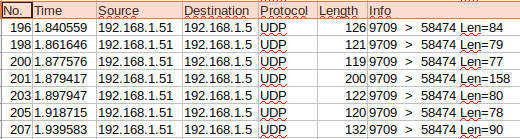
\includegraphics[width=\textwidth]{img/confronto-headeri}
\captionof{figure}{La colonna \emph{Length} mostra la lunghezza totale, nella colonna \emph{Info} è mostrata la lunghezza della sezione dati: 42 byte vengono utilizzati per l'header}
\end{minipage}
\newpage
Come è già stato reso noto da precedenti studi nel campo, è possibile distinguere le due fasi principali di una chiamata Skype: la fase di \textsl{ringing}, in cui viene stabilita la connessione fra due (o più) utenti e la fase di \textsl{conversazione}.\newline Si possono notare differenze sia nella \emph{quantità} di pacchetti inviati che nella loro dimensione: durante la fase di \textsl{ringing} di una chiamata fra due utenti, l'utente A (il chiamante) invia in un primo momento tre pacchetti di dimensione fissa contemporaneamente, rispettivamente (comprensivi di header) di 114, 138 e 142 byte all'utente B (il chiamato). Dopodiché invierà altri due pacchetti con un intervallo di 20 secondi, di 130 byte. L'utente B risponde al primo pacchetto ricevuto inviando 138 byte, 114 per i successivi. Tutti gli altri pacchetti inviati vengono utilizzati per contattare i supernodi per poter stabilire una connessione fra le due entità. In ogni caso il numero di pacchetti trasmessi in questa fase è esiguo rispetto a quello nella seconda fase.\newline
Appena l'utente B accetta la chiamata il rate di trasmissione aumenta in modo considerevole, come mostrato nella Figura 2. Questo è dovuto al fatto che Skype non supporta la soppressione dei silenzi e quindi vengono costantemente inviati e ricevuti pacchetti nel corso della chiamata. È possibile, tuttavia, distinguere le fasi silenziose da quelle parlate in quanto il protocollo utilizzato non invia una quantità costante di byte.\newline\newline\newline\newline
\begin{minipage}{\linewidth}
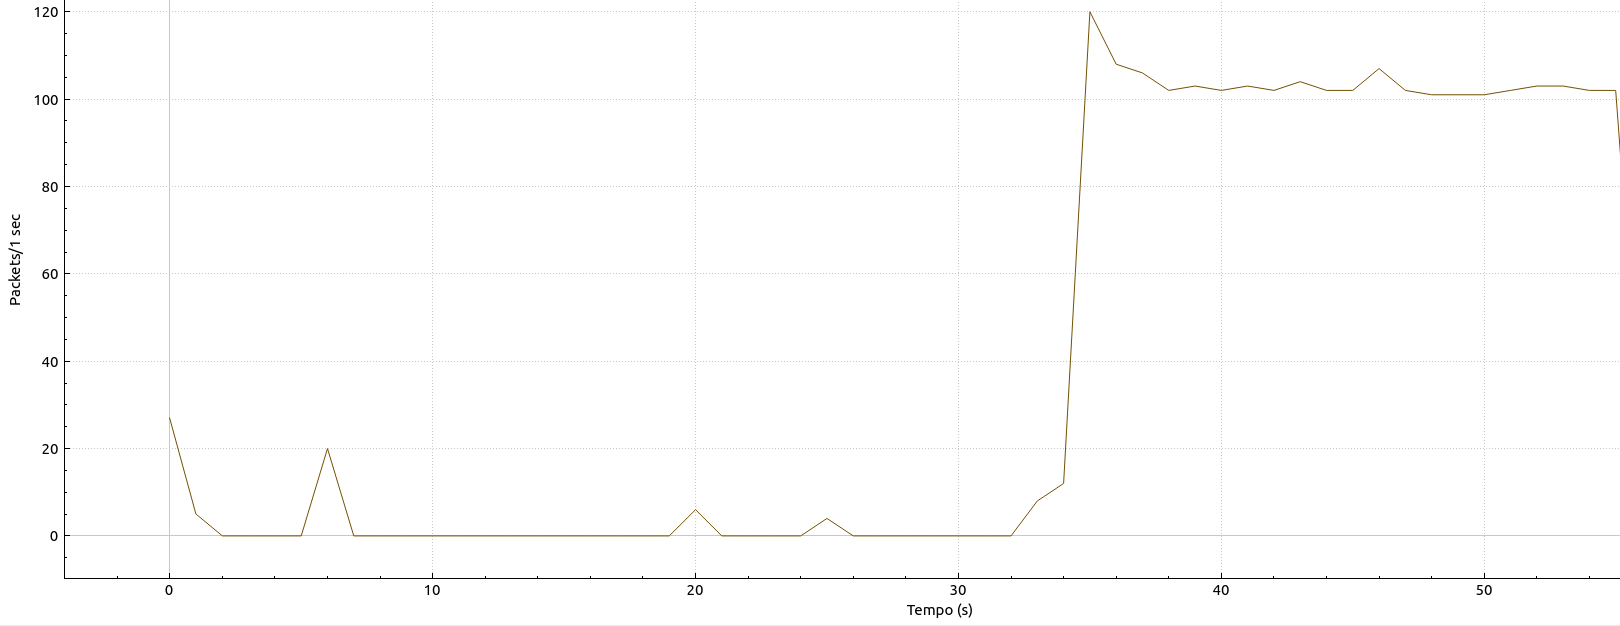
\includegraphics[width=1.2\textwidth,keepaspectratio]{img/packet-rate}
\captionof{figure}{In figura è possibile osservare la differenza di quantità di pacchetti inviati nelle fasi di ringing e di conversazione}
\end{minipage}
\section{Analisi delle chiamate Skype}
In questa sezione verranno discussi i risultati ottenuti dal monitoraggio delle chiamate Skype fra due utenti e più. In una prima parte verranno trattate le conversazioni effettuate usando messaggi pre-registrati e libere, grazie all'ausilio del software open source \emph{Skypegrep}. Saranno riportati dati statistici come media e varianza della lunghezza dei pacchetti e saranno argomentati i risultati ottenuti a seguito dell'analisi. Infine verranno trattate le videochiamate e le conferenze Skype.\newline

\subsection{Conversazione fra due utenti}

I dati che sono stati raccolti in questi esperimenti non si discostano dai risultati di esperimenti precedenti: nelle fasi \textbf{silenziose} la lunghezza media dei pacchetti è risultata $\bar x\ = 127 $
con deviazione standard $\sigma = 6 $, nelle fasi di \textbf{conversazione} invece la dimensione aumenta in modo significativo, portando la media a $\bar x\ = 149 $ e deviazione standard $\sigma = 9$.\newline (I dati riportati si basano sull'analisi di \emph{tutti} gli esperimenti effettuati)\newline\newline
Durante l'osservazione è stato notato l'invio di un pacchetto di dimensione fissa, inviato a intervalli di tempo irregolari, la cui dimensione è costante durante una conversazione. La presenza di questo pacchetto, probabilmente dovuta al protocollo utilizzato da Skype, è stata utile quando sono state condotte le analisi sulle videochiamate e le conferenze. È inoltre possibile filtrarli facilmente data la lunghezza costante.\newline
\begin{minipage}{\linewidth}
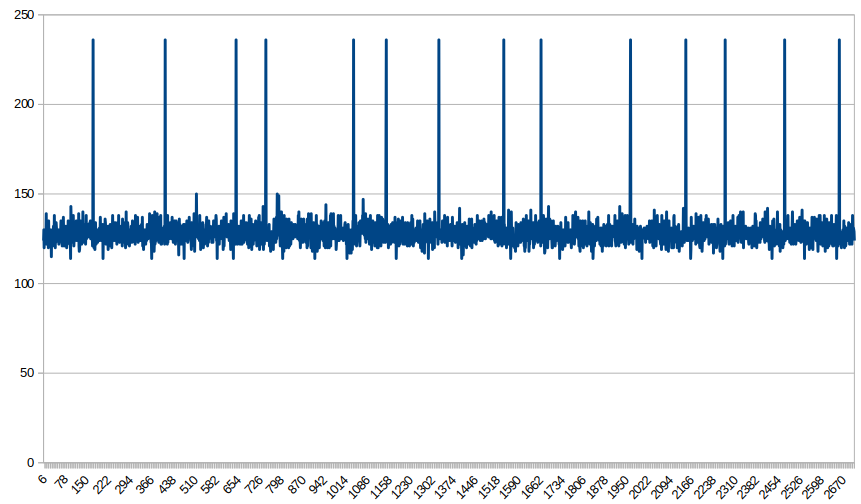
\includegraphics[width=\textwidth,keepaspectratio]{img/pacchetti236}
\captionof{figure}{Istantanea di una fase silenziosa: vengono inviati pacchetti molto lunghi a intervalli irregolari.}
\end{minipage}\newline\newline\newline

\subsection{Riconoscimento rumori esterni}

Uno degli obiettivi di questo progetto è stato quello di capire se fosse possibile identificare eventuali rumori esterni in una conversazione (sirena di un'ambulanza, colpo di tosse\dots), tuttavia nel corso di questi esperimenti non è stato \emph{sempre} possibile rilevare questo tipo di disturbi a causa di diversi fattori che saranno elencati di seguito.\newline
Prima di proseguire con la trattazione è doveroso andare ad analizzare in che modo Skype codifica in bit i suoni catturati.\newline\newline Skype utilizza un codec audio proprietario, SILK, a bitrate variabile. Il bitrate è la quantità di bit con cui i suoni vengono codificati al secondo: utilizzando codec a bitrate variabile (VBR) è possibile che uno stesso suono venga codificato a bitrate differenti, producendo quindi pacchetti di dimensione differente. Inoltre, il protocollo di crittografia utilizzato mantiene inalterata la lunghezza della codifica audio-bit, questo fatto è stato utilizzato dal gruppo \emph{MDSec} per identificare le frasi pronunciate dagli utenti.\newline\newline
Al momento, l'unico tipo di attacco  in grado di riconoscere le frasi pronunciate da un utente sfrutta questa proprietà: una stessa frase ripetuta in momenti diversi verrà trasmessa sulla rete in pacchetti di dimensione differente (ma simile), mentre frasi differenti produrranno sequenze diverse per quanto riguarda la lunghezza dei pacchetti. Per riconoscere le frasi pronunciate viene utilizzando quindi l'Hidden Markov Model che modella il processo di codifica (per maggiori informazioni si rimanda a \cite{bibitem1}). L'approccio con cui si effettua la rilevazione di frasi pronunciate è indipendente dall'utente (impedendo di riconoscerne l'identità) a meno di notevoli differenze nella pronuncia di alcune parole/frasi.
\newline
Con questa premessa risulta chiaro quanto possa essere difficile captare eventuali rumori esterni durante una conversazione osservando solamente la dimensione dei pacchetti: piccole variazioni potrebbero sì essere dovute, ad esempio, a un colpo di tosse da parte dell'utente ma anche a una differente codifica della frase pronunciata. Tuttavia in alcuni casi, se tali rumori sono prodotti dall'utente stesso, si è potuto osservare un'alterazione nell'andamento della funzione che misura la lunghezza dei pacchetti.\newline\newline
Per l'esperimento sono state registrate tre frasi differenti, prima in modo pulito e una seconda volta aggiungendo due evidenti colpi di tosse a metà della frase, interrompendo quindi il regolare flusso di parole, dopodiché è stata pronunciata la parte mancante della sentenza. È stato quindi osservato l'andamento della dimensione dei pacchetti e sono stati eseguiti dei test con l'ausilio di \emph{Skypegrep}.\newline
Analizzando i dati raccolti effettuando gli esperimenti con frasi registrate, si è potuto osservare come la media della lunghezza dei pacchetti nelle frasi con i colpi di tosse fosse \emph{sempre} maggiore di 3.5$\pm$0.5 byte rispetto alle frasi pronunciate in condizioni ideali (non sono state invece trovate differenze rilevanti per quanto riguarda la varianza, nè per il rate di trasmissione).\newline
In alcuni casi è stato inoltre possibile, sia graficamente, sia andando ad osservare l'istante di tempo in cui avviene il colpo di tosse, osservare una diminuzione della lunghezza dei pacchetti seguito da un picco repentino, tuttavia questo comportamento non si è manifestato in tutti gli esperimenti, impedendo quindi di fornire una regola generale per il riconoscimento, inoltre skypegrep è stato in grado di riconoscere la frase pronunciata nell'80\% dei casi (con tosse) proprio per il fatto che piccole differenze fra i due pattern potrebbero essere dovute a una codifica con bitrate differente.\newline\newline

Nelle immagini riportate di seguito si può notare delle differenze nei primi 2 grafici (relativi ad una stessa frase prima senza, poi con il colpo di tosse), mentre questo non accade nella seconda coppia di figure.\newline
\begin{minipage}{\linewidth}
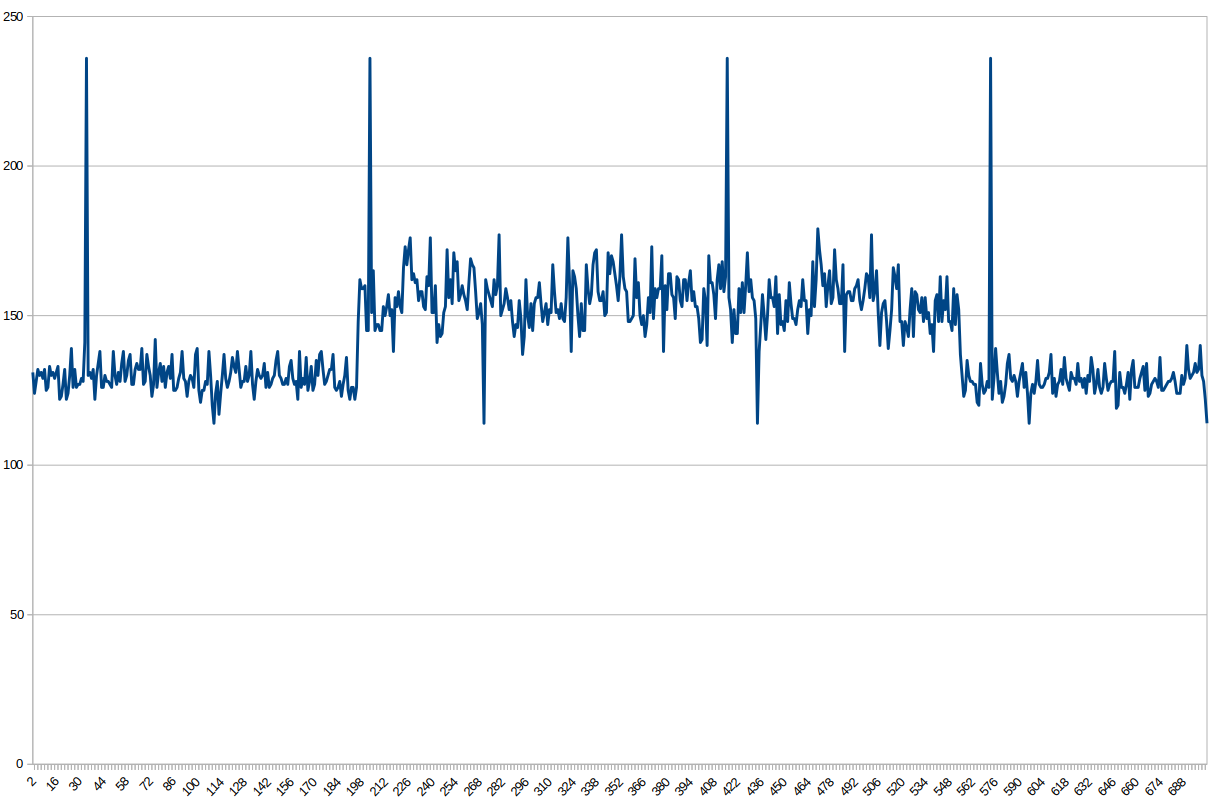
\includegraphics[width=\textwidth,keepaspectratio]{img/SenzaTosse}
\captionof{figure}{Grafico della prima frase senza colpo di tosse.}
\end{minipage}
\begin{center}
$\bar x\ = 145 $, $\sigma = 15 $
\end{center}


\begin{minipage}{\linewidth}
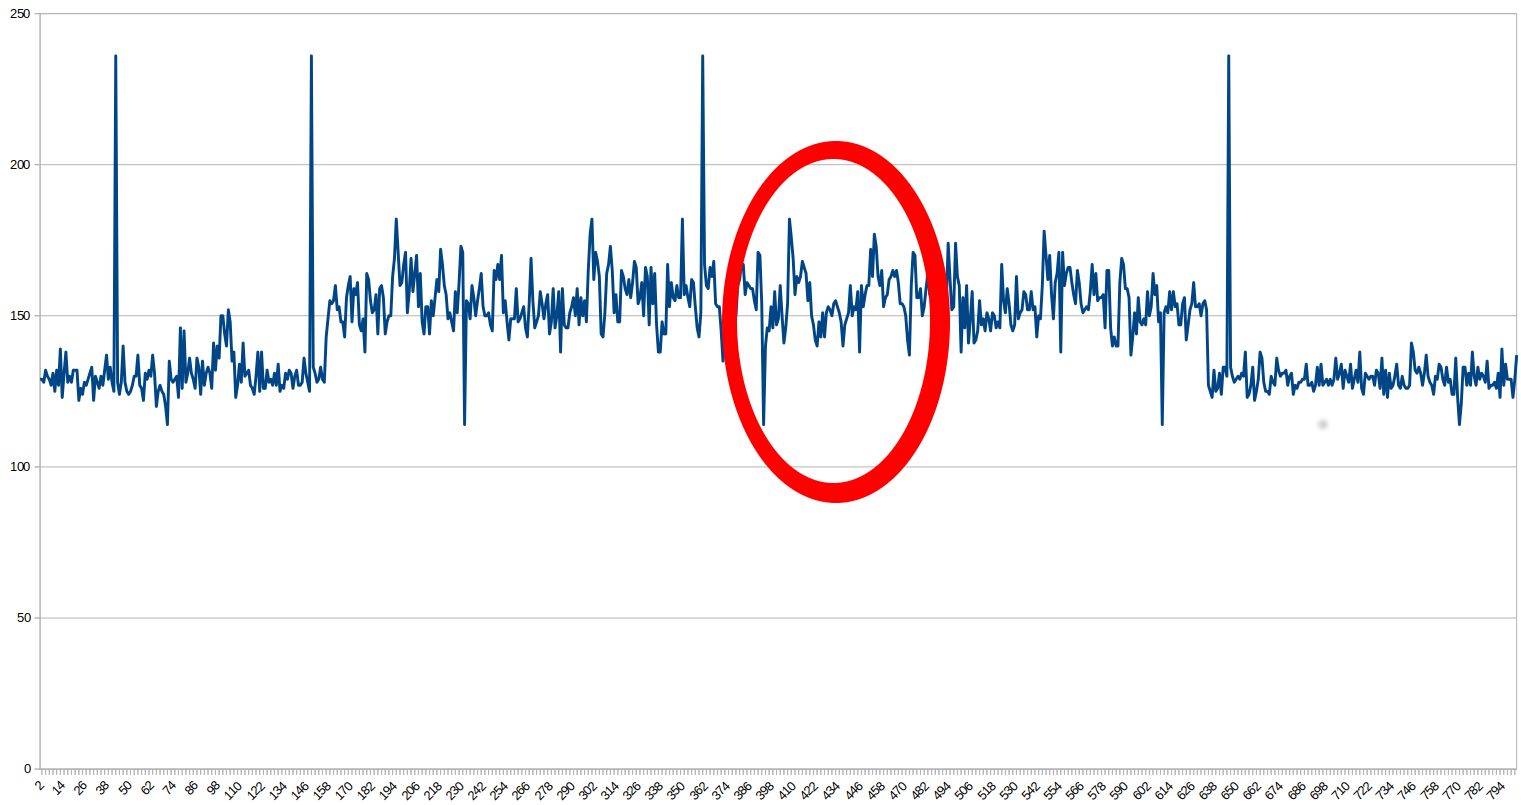
\includegraphics[width=\textwidth,keepaspectratio]{img/ColpoTosse}
\captionof{figure}{Grafico della prima frase con colpo di tosse, è possibile notare dal grafico il momento in cui è avvenuto il colpo di tosse.}
\end{minipage}
\begin{center}
$\bar x\ = 148 $, $\sigma = 14.5 $
\end{center}

\begin{minipage}{\linewidth}
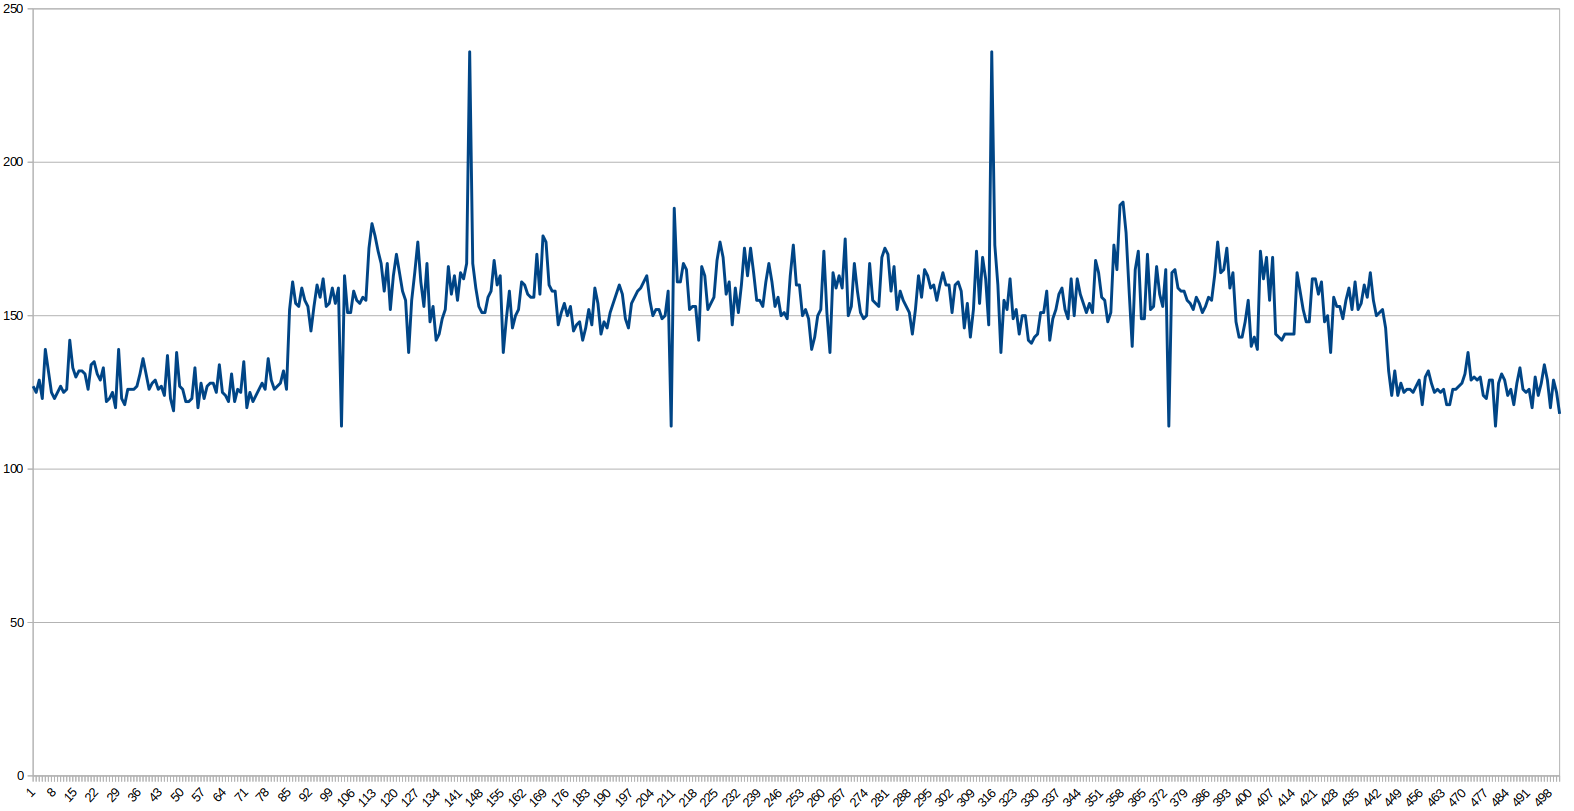
\includegraphics[width=\textwidth,keepaspectratio]{img/GraficoSenzaTosse2}
\captionof{figure}{Grafico della seconda frase senza colpo di tosse.}
\end{minipage}
\begin{center}
$\bar x\ = 146 $, $\sigma = 15 $
\end{center}


\begin{minipage}{\linewidth}
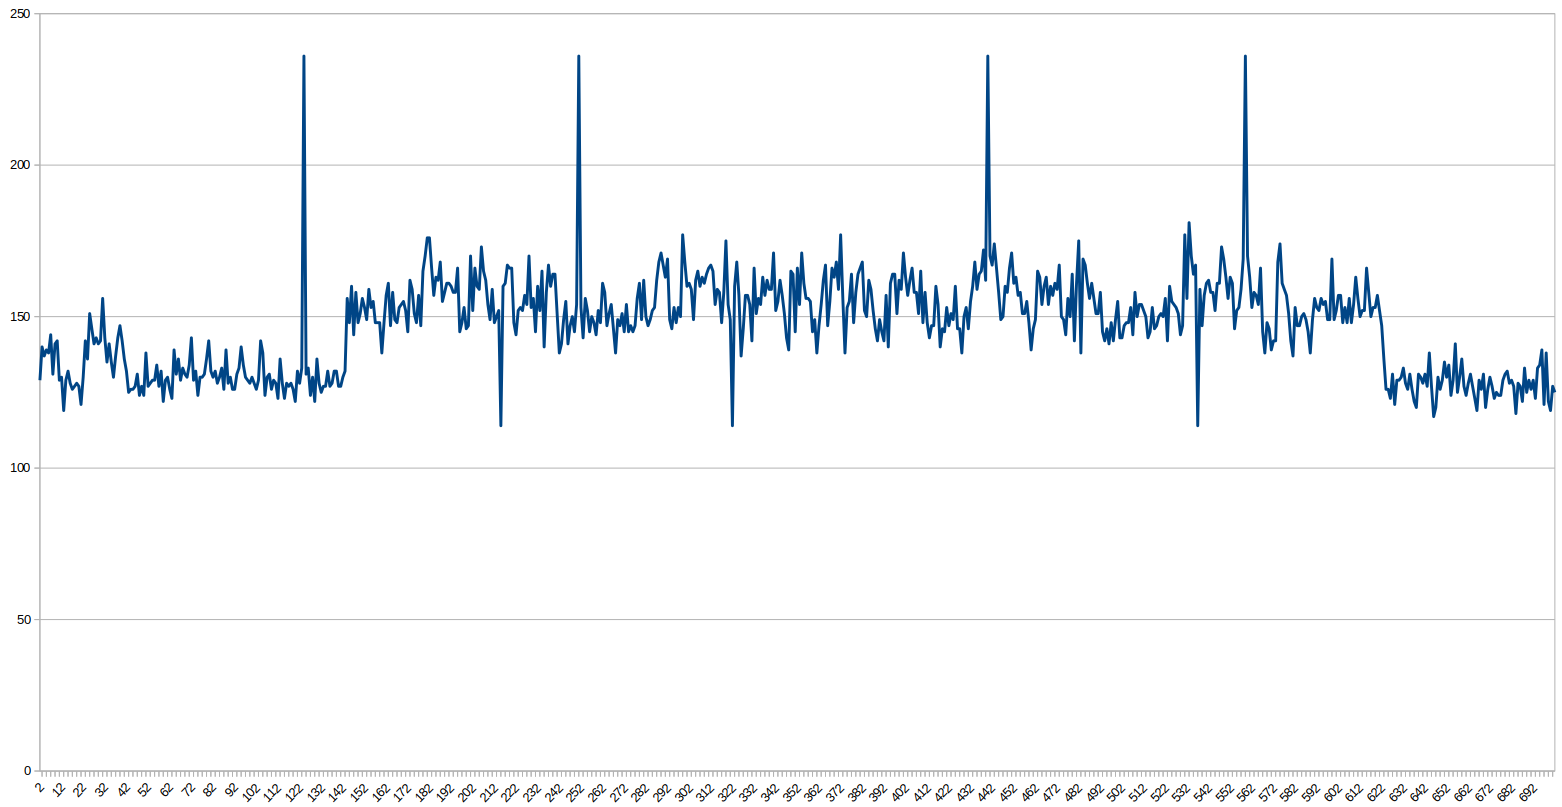
\includegraphics[width=\textwidth,keepaspectratio]{img/ColpoTosse2}
\captionof{figure}{Grafico della seconda frase con colpo di tosse, non si è in grado di attribuire le piccole variazioni a un disturbo o a una codifica con bitrate differente.}
\end{minipage}
\begin{center}
$\bar x\ = 149 $, $\sigma = 14.5 $
\end{center}

Nonostante non sia stato possibile fornire un criterio per il riconoscimento di eventuali disturbi "istantanei" nel segnale audio, è stato trovato un risultato interessante per quanto riguarda rumori di sottofondo costanti, come ad esempio della musica o il rumore di un aspirapolvere.\newline
Nel caso in cui queste fonti di disturbo si trovassero vicino al microfono è possibile notare un cambiamento nella lunghezza media dei pacchetti, a patto di aver osservato sufficientemente l'andamento della suddetta. Gli esperimenti per queste casistiche sono stati effettuati ripetendo le stesse frasi prima in condizioni di silenzio, successivamente con della musica in sottofondo.\newline Nel primo caso i dati rilevati sono risultati in linea con tutti quelli visti fino ad ora, nel secondo caso invece abbiamo potuto assistere a un innalzamento della lunghezza media. In particolare facendo una media sulla \emph{totalità} dei pacchetti, nelle conversazioni effettuate in condizioni di silenzio la media è risultata essere di 144 con una deviazione standard di 16, mentre nelle conversazioni con un disturbo di sottofondo la media si alza a 153 con una deviazione standard più bassa, pari a 14. L'abbassamento della deviazione standard può essere dovuto al fatto che anche nelle fasi in cui l'utente non parla vengano catturati i suoni dovuti al disturbo in sottofondo, alzando quindi la media totale e provocando una variazione minore fra i pacchetti trasmessi nelle fasi silenziose e in quelle di conversazione.\newline\newline

Per concludere questo paragrafo:

\begin{itemize}
\item È possibile in \emph{alcuni} casi riconoscere un'interruzione della frase pronunciata (a causa di un colpo di tosse o di eventuali tic \underline{evidenti}) dopo aver effettuato una profilazione dell'utente, se le frasi non disturbate vengono sempre ripetute in modo \underline{identico}.
\item È sempre possibile capire se l'utente si trova in un contesto rumoroso in quanto si notano variazioni evidenti della media e della deviazione standard.
\end{itemize}

\section{Videochiamate e conferenze}

In questa sezione verranno mostrati i risultati ottenuti conducendo indagini su videochiamate e conferenze Skype. Gli obiettivi posti sono:

\begin{itemize}
\item Identificare se l'utente sta partecipando ad una conferenza
\item Identificare se l'utente sta effettuando una videochiamata
\item Isolare i pacchetti audio da quelli video
\end{itemize}

Sorprendentemente sono stati ottenuti dei risultati significativi per tutti gli obbiettivi proposti.

\subsection{Analisi delle videochiamate}

Osservando il traffico di rete di un utente, è possibile capire se questo sta effettuando una chiamata o una videochiamata? È possibile identificare quale parte dei pacchetti sta inviando segnali audio piuttosto che video?\newline
Le videochiamate Skype forniscono risultati \textbf{evidentemente} differenti da quelli ottenuti analizzando delle normali chiamate, sia in termini di traffico di rete (quantità di pacchetti inviati al secondo) sia in termini di lunghezza dei pacchetti.\newline
Questo viene dal fatto che i pacchetti audio e video sono inviati separatamente, costringendo la rete a inviarne un numero molto maggiore, aumentando considerevolmente il rate di trasmissione. La differenza fra una normale chiamata e una con video è evidente anche graficamente e media e varianza della lunghezza dei pacchetti sono di gran lunga superiori rispetto a quanto visto fin'ora.

\begin{center}

\begin{minipage}{\linewidth}
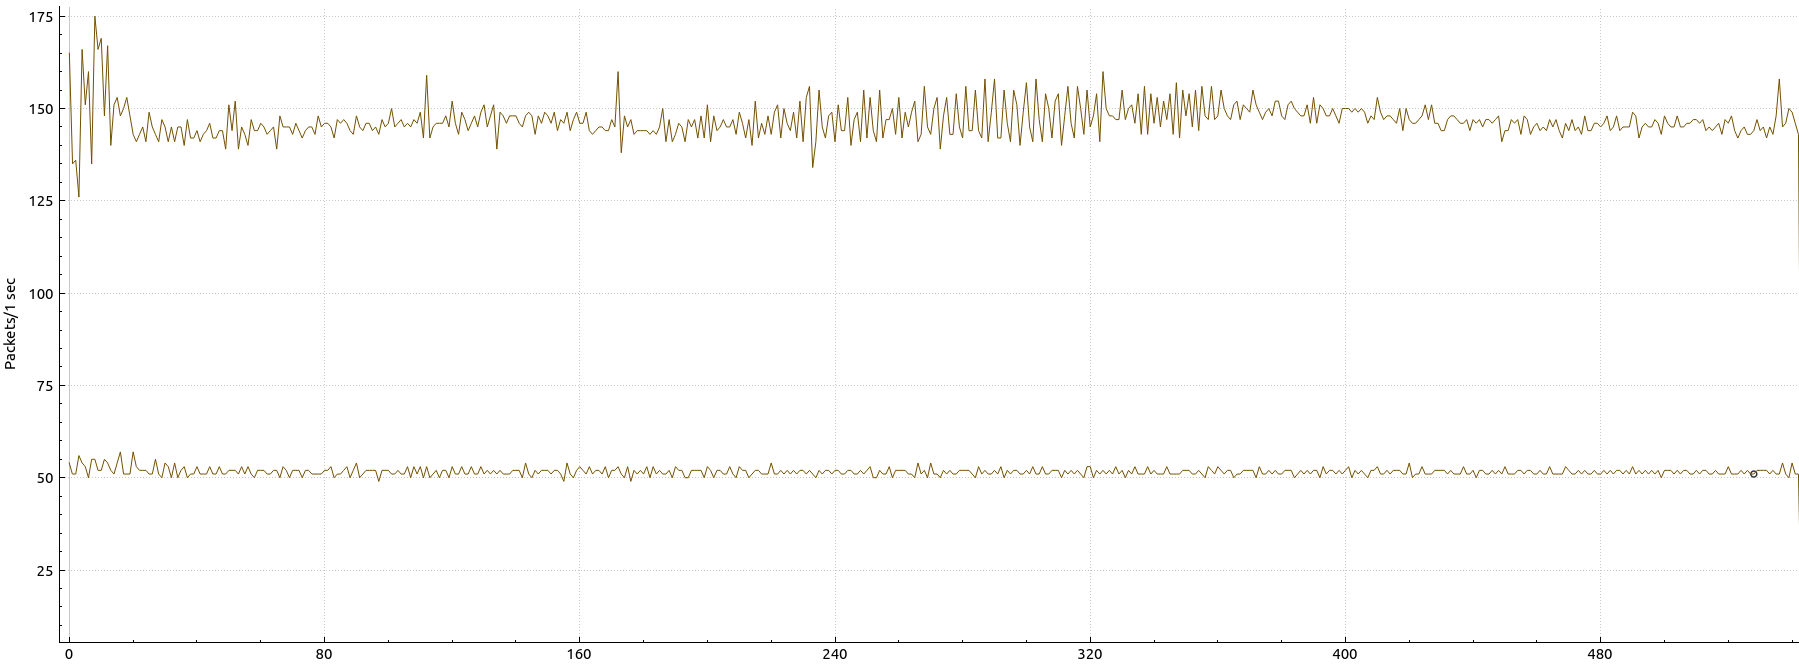
\includegraphics[width=1.2\textwidth,height = 8cm]{img/videochiamata-packet-rate}
\captionof{figure}{Numero di pacchetti trasmessi al secondo. Come è possibile vedere dal grafico l'utente che utilizza la videocamera invia una media di 100 pacchetti in più al secondo.}
\end{minipage}
\end{center}

Negli esperimenti condotti la media di pacchetti trasmessi al secondo è risultata di 148.7 per le videochiamate, contro i 49 delle chiamate regolari.\newline
Possiamo notare sostanziali differenze anche per quanto riguarda la lunghezza dei pacchetti: se nelle normali chiamate audio la dimensione media (considerando insieme fasi silenziose e di conversazione) si attestava fra i 140 e i 155 byte, nelle videochiamate è possibile notare come questa aumenti in modo considerevole, portando la lunghezza media a 713 byte, con una deviazione standard molto elevata, pari a 445.\newline
Una deviazione standard così alta è dovuto al fatto che la dimensione dei \emph{pacchetti video} sia di gran lunga superiore ai pacchetti audio (circa un'ordine di grandezza di differenza!). Infatti la media di questi si attesta sui 1030 byte, contro la media di 140-150 dei pacchetti audio.\newline\newline
Nel paragrafo sull'analisi delle chiamate Skype fra due utenti è stato osservato l'invio di un pacchetto di dimensione fissa (237 byte). La presenza di un gran numero di pacchetti di questa dimensione è stato osservato anche nelle videochiamate, è stato pertanto ipotizzato che tale dimensione potesse essere una sorta di spartitraffico fra i pacchetti audio e quelli video.\newline Sorprendentemente tale intuizione si è rivelata esatta: filtrando i pacchetti di dimensione inferiore a 237 è possibile riscontrare delle similitudini fra l'andamento dei pacchetti filtrati e quello osservato nelle chiamate senza video. Calcolando la media dei pacchetti di lunghezza superiore a 127 byte (questo bound è stato scelto basandosi sulla media della lungheza dei pacchetti nelle fasi silenziose) e inferiore a 237, questa è risultata in linea con i dati ottenuti dalle rilevazioni effettuate nella sezione 2.2 ottenendo una media (sulla totalità degli esperimenti) di 150 byte di lunghezza per le fasi di conversazione. Nelle due immagini seguenti viene proposto un confronto fra l'andamento della dimensione dei pacchetti prima e dopo aver applicato il filtro sulla lunghezza.

\begin{center}

\begin{minipage}{\linewidth}
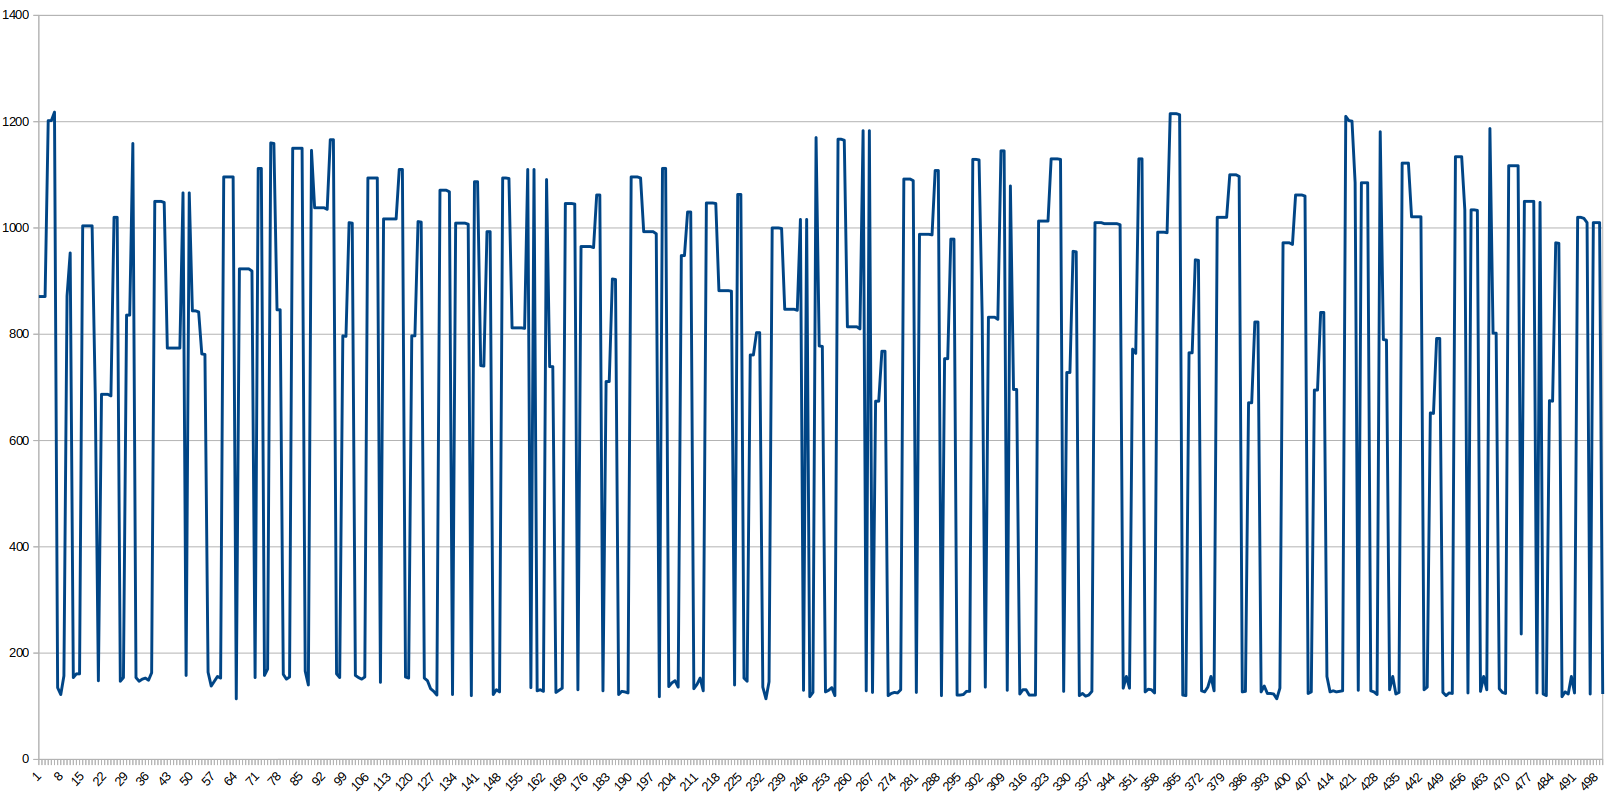
\includegraphics[width=\textwidth,keepaspectratio]{img/videochiamata-non-filtrata}
\captionof{figure}{In figura viene mostrata la dimensione dei pacchetti senza applicare alcun filtro. Si nota come l'andamento sia altamente irregolare, in linea con la alta deviazione standard calcolata.}
\end{minipage}

\begin{minipage}{\linewidth}
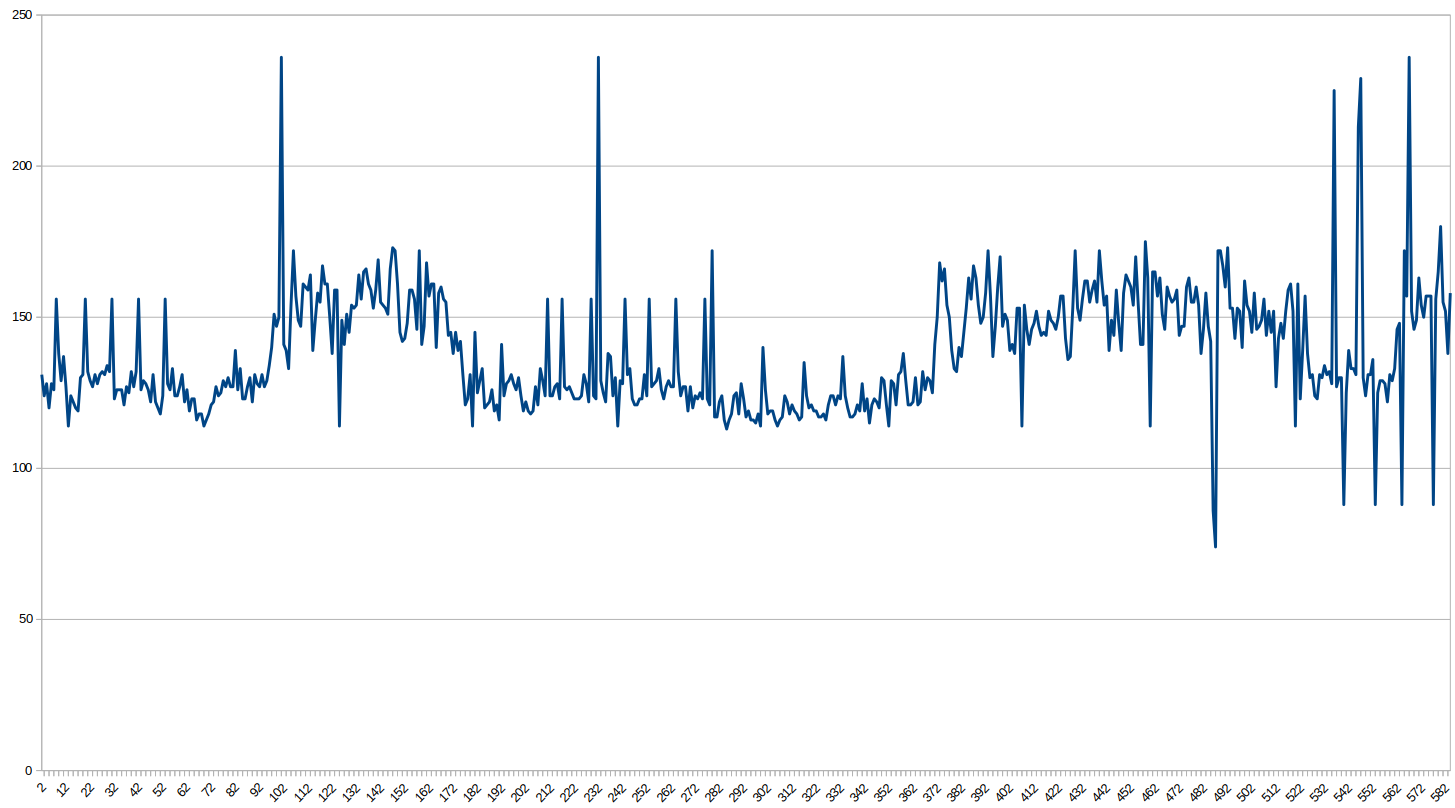
\includegraphics[width=\textwidth,keepaspectratio]{img/Filtro-audio-videochiamata}
\captionof{figure}{Qui viene applicato il filtro sulla lunghezza dei pacchetti: è possibile osservare un comportamento in linea con i dati ottenuti nel capitolo precedente sull'analisi delle chiamate.}
\end{minipage}
\end{center}

Per confermare l'ipotesi sono stati effettuati dei test con Skypegrep, il quale è riuscito a riconoscere le frasi pronunciate in 8 casi su 10 (gli sviluppatori stessi affermano che non sia possibile avvere un'accuratezza del 100\% e che questa si attesta fra l'80\% e il 90\%).\newline\newline
A seguito di questa analisi possiamo trarre due importanti conclusioni: non solo è possibile capire quando un utente attiva la videocamera semplicemente analizzando il traffico di rete (si notano dei picchi non indifferenti) ma è anche possibile isolare i pacchetti audio da quelli video!\newline In questo modo risulta possibile intercettare e riconoscere le frasi pronunciate anche in caso di videochiamata fra due utenti.\newline Sfortunatamente ancora non sono stati trovati metodi per decifrare i pacchetti video, tuttavia questo risultato può essere utilizzato come punto di partenza per l'identificazione e una successiva decifrazione.

\subsection{Analisi delle conferenze}

In questa sezione verranno analizzate le conferenze skype fra 3 utenti e in che modo sia possibile riconoscerle. Per condurre questi esperimenti è stata prima effettuata una normale chiamata fra due utenti, a cui poi veniva aggiunto un terzo per creare una conferenza Skype.\newline\newline
Inanzitutto ricordiamo che Skype utilizza una comunicazione peer-to-peer, in cui due (o più) utenti per mettersi in comunicazione contattano un super nodo (tipicamente un altro utente Skype, scelto in base a dei criteri come la banda disponibile e la posizione geografica) per mettersi in contatto fra di loro.\newline
Il fatto interessante che è stato osservato durante questi esperimenti è che la gestione della conferenza è completamente delegata a un super nodo che si occupa di coordinare i partecipanti.\newline È stato possibile notarlo in quanto gli utenti non inviavano pacchetti ai reciproci indirizzi IP, bensì a indirizzi non noti situati in altre parti del mondo (Olanda, USA\dots).\newline In ogni caso, a differenza dei precedenti esperimenti, non è stato possibile ottenere risultati soddisfacenti, in quanto il comportamentento sia in termini di packet rate che di lunghezza è risultato alquanto irregolare.\newline\newline

Un primo risultato ottenuto è dato dal fatto che sia possibile notare il momento in cui viene effettuata la conferenza. Filtrando i pacchetti inviati dall'indirizzo IP "192.168.1.52" che all'inizio della chiamata (che ricordiamo essere fra due utenti) inviava all'indirizzo "192.168.1.10" si è potuto notare come ad un certo punto la comunicazione fra i due venisse interrotta e entrambi gli utenti iniziassero a comunicare con un indirizzo sconosciuto "52.166.75.118".

\begin{center}
\begin{minipage}{\linewidth}
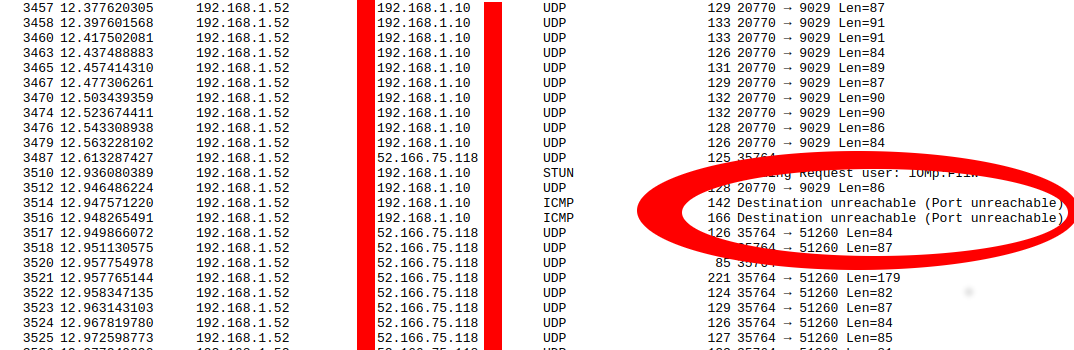
\includegraphics[width=\textwidth,keepaspectratio]{img/conferenza}
\captionof{figure}{In figura è possibile notare il momento in cui la connessione fra i due utenti viene chiusa e questi cominciano a comunicare con il super nodo.}
\end{minipage}
\end{center}

Pertanto, guardando i destinatari dei pacchetti è possibile capire il momento in cui viene iniziata una conferenza Skype.\newline
Andando ad analizzare dimensione e frequenza dei pacchetti si può notare come quest'ultima inizi a seguire un andamento altamente irregolare nel momento in cui ha inizio la conferenza. Questo comportamento si può attribuire al fatto che la maggior parte del lavoro venga svolto dal super nodo che si occupa di coordinare i partecipanti.

\begin{center}
\begin{minipage}{\linewidth}
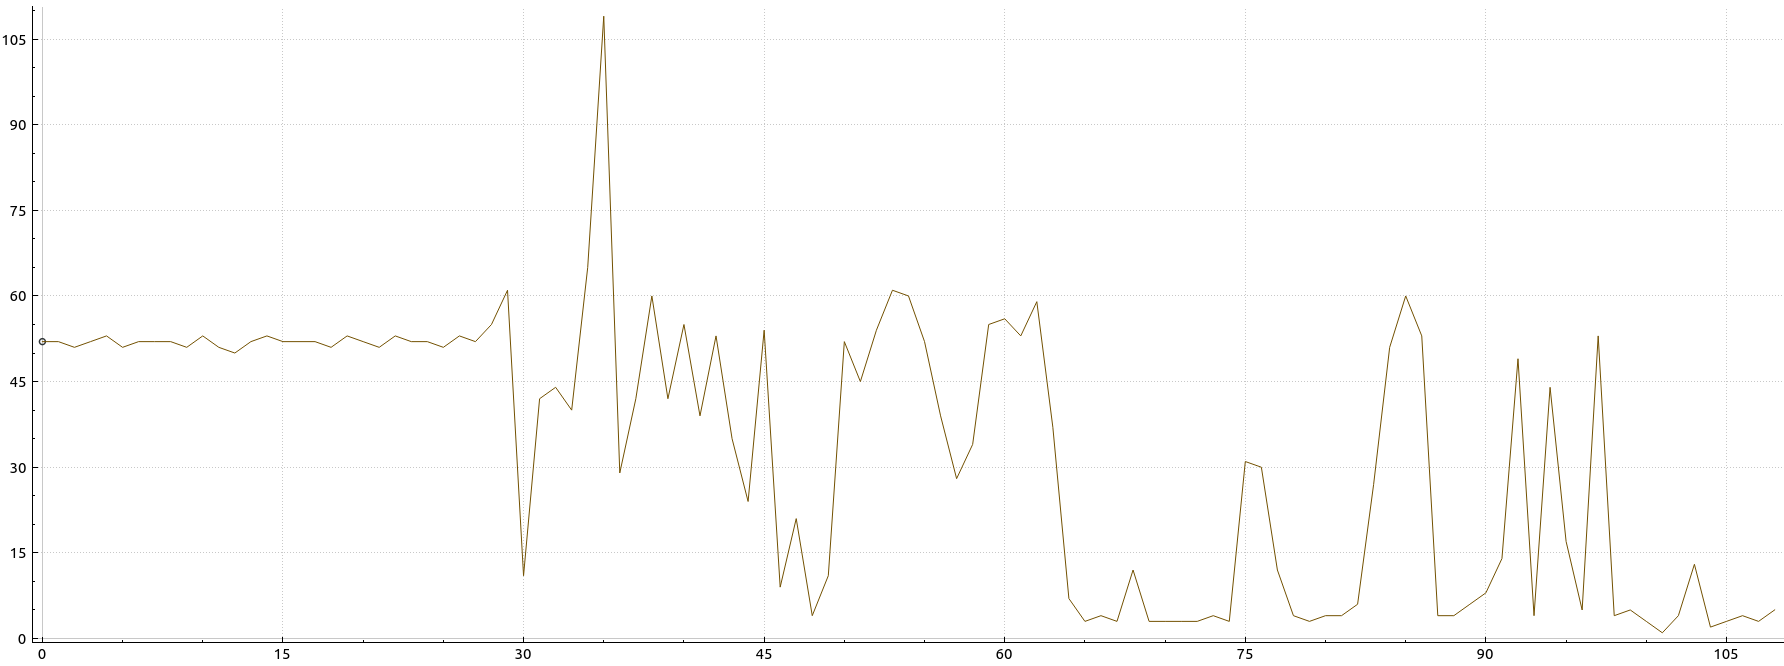
\includegraphics[width=\textwidth,keepaspectratio]{img/inizio-conferenza}
\captionof{figure}{In figura è possibile notare il momento in cui la connessione fra i due utenti viene chiusa e questi cominciano a comunicare con il super nodo.}
\end{minipage}
\end{center}

È possibile notare differenze anche nella lunghezza media dei pacchetti inviati, nonostante queste non siano evidenti come nel caso delle videochiamate ad esempio.\newline
Nel corso delle rilevazioni la media sperimentale è risultata essere pari a 170 (circa 30 byte sopra alla media delle conversazioni normali) con una deviazione standard di 165. Purtroppo, a differenza dei casi precedenti, è risultato difficile trovare delle regolarità nell'andamento della lunghezza dei pacchetti. Inanzitutto vengono inviati molti più pacchetti di piccole dimensioni (sotto ai 100 byte), mentre la dimensione del pacchetto "spartitraffico" di 237 byte, rilevato sia nelle conversazioni normali che nelle videochiamate, si alza a 957.\newline
Per tentare di riconoscere quindi quali fossero i pacchetti in cui veniva codificato l'audio sono stati presi un bound superiore di 250 byte, e uno inferiore di 127 (basandosi sulla media calcolata nei casi precedenti). Filtrando i dati in questo modo è stato ancora una volta possibile trovare un andamento regolare per la lunghezza dei pacchetti in linea con le frasi pronunciate dall'utente e con i risultati visti fin'ora, tuttavia il riconoscimento delle frasi è risultato difficile in quanto abbiamo più variazione sulla dimensione dei pacchetti, probabilmente dovuto al protocollo di coordinazione fra gli utenti. Anche eseguendo dei test con Skypegrep è stato possibile identificare le frasi pronunciate solamente fra il 40\% e il 60\% dei casi.

\begin{center}
\begin{minipage}{\linewidth}
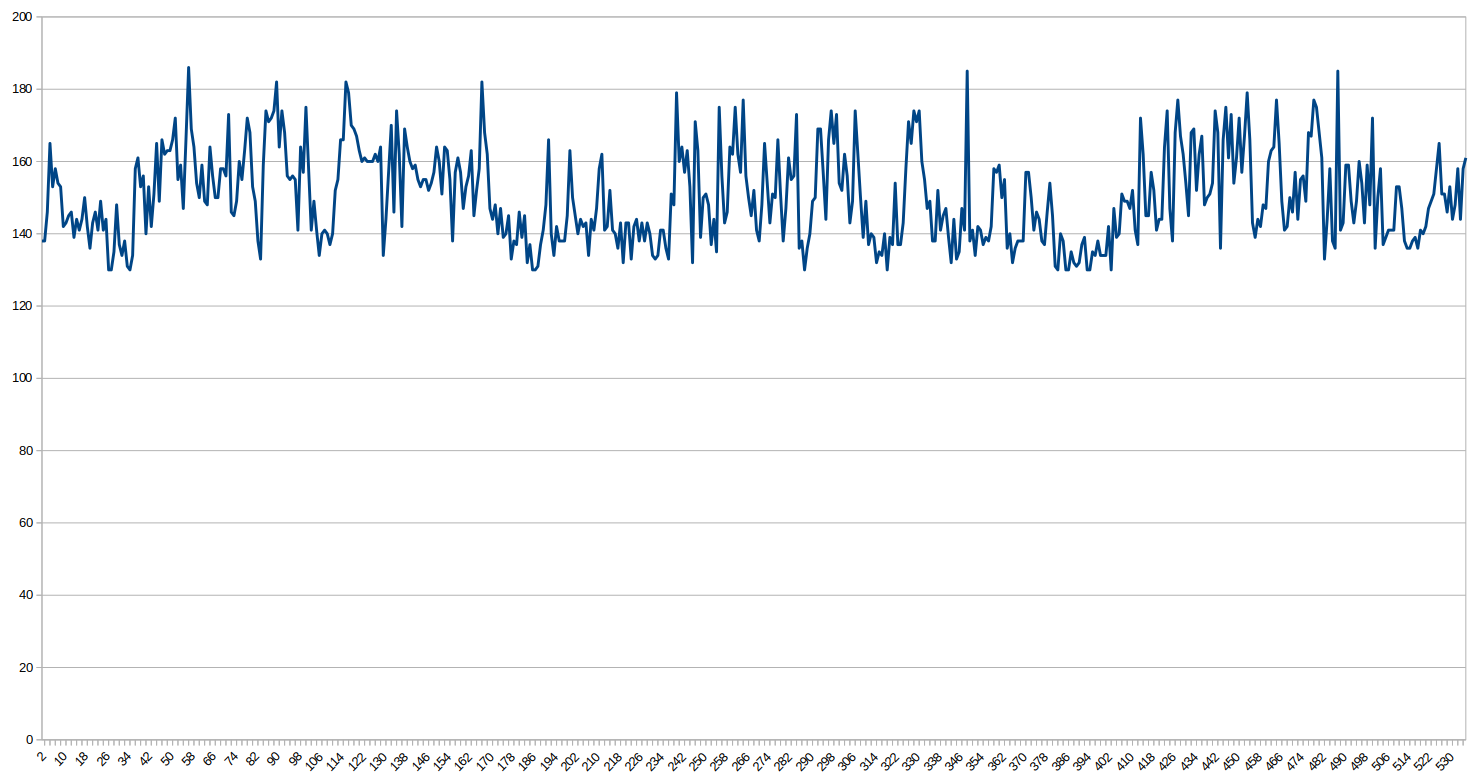
\includegraphics[width=\textwidth,keepaspectratio]{img/pacchetti-conferenza}
\captionof{figure}{Nel grafico è possibile vedere come anche nei momenti di silenzio vengano inviati pacchetti di dimensione maggiore alla media calcolata fin'ora, disturbandone l'andamento.}
\end{minipage}
\end{center}

\section{Skypegrep}

Prima di concludere il lavoro, di seguito verrà fatta una rapida panoramica sul software Skypegrep, unico software open-source che al momento è in grado di sferrare attacchi al VoIP osservando unicamente le sequenze di pacchetti trasmessi e che è stato molto utilizzato in fase di sperimentazione.\newline
Una trattazione completa sull'argomento richiederebbe uno studio approfondito che esula dagli scopi di questa relazione, comunque sia si ritiene utile spiegare in breve come funziona il software e in che modo questo analizzi il traffico di rete generato da Skype.\newline\newline
Come accennato in precedenza, tale attacco si basa sull'utilizzo dell'\emph{Hidden Markov Model} con cui è possibile modellare le frasi pronunciate da un utente. Un'HMM è una catena di Markov in cui gli stati non sono direttamente osservabili e le transizioni da uno stato all'altro avvengono in modo statisticamente indipendente.\newline
Viene eseguita inizialmente una frase di \emph{training} in cui si insegna al software a riconoscere una determinata frase (i.e. una sequenza di pacchetti), dopodiché, una volta effettuata la profilazione, si analizzano le sequenze di pacchetti oggetto di studio.\newline Partendo dallo stato iniziale dell'HMM, il software cambia stato attribuendo una probabilità alle transizioni che viene calcolata in fase di training. Quando viene raggiunto uno stato finale si è in grado di dire (con un'affidabilità fra l'80\& e il 90\%) se nella sequenza di pacchetti analizzata sia presente o meno la frase con cui è stata eseguita la fase di training.\newline
Come menzionato anche nel \textsl{paper} \cite{bibitem1} non è possibile fare a meno di utilizzare un modello probabilistico per effettuare questo tipo di attacco: a causa dei codec utilizzati per la cattura e la trasmissione dell'audio le sequenze di pacchetti IP osservati non saranno \textbf{mai} uguali, neanche per una frase ripetuta in modo identico dallo stesso utente (questo è uno dei motivi per cui non si è stati in gradi di riconoscere rumori come il colpo di tosse).\newline
Un aspetto interessante che è stato notato durante lo studio è che nonostante i file di training siano stati generati utilizzando delle forti restrizioni (i.e. frasi registrate, intervalli di 5-10 secondi di silenzio fra una sentenza e l'altra), il software è stato in grado di riconoscere nella maggior parte dei casi le frasi pronunciate anche in conversazioni libere.

\begin{center}
\begin{minipage}{\linewidth}
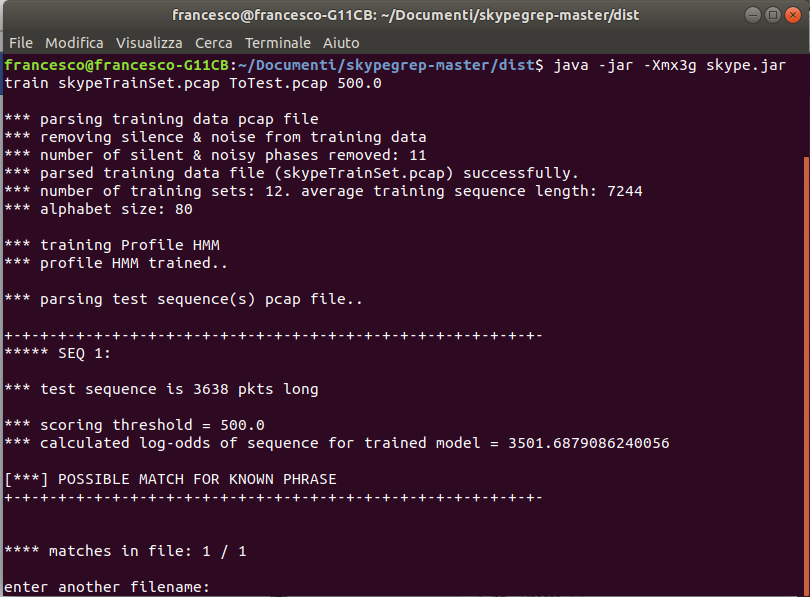
\includegraphics[width=\textwidth,keepaspectratio]{img/skypegrep}
\captionof{figure}{Il file di training è composto da una frase registrata ripetuta più volte, il test è stato poi effettuato su un file .pcap generato da una conversazione libera fra due utenti. Si ha il riconoscimento quando il software ottiene un punteggio maggiore di 500.}
\end{minipage}
\end{center}